\documentclass[letter, 10pts]{article}
\usepackage[monocolor]{../math232/ahsansabit}
\usepackage[]{float}
\usepackage{tikz}
\usepackage{tikz-3dplot}
\usepackage[outline]{contour} % glow around text
\usepackage{xcolor}
\usepackage{pdfpages}
\usepackage{physics}
\usepackage{multicol}
\colorlet{veccol}{green!50!black}
\colorlet{projcol}{blue!70!black}
\colorlet{myblue}{blue!80!black}
\colorlet{myred}{red!90!black}
\colorlet{mydarkblue}{blue!50!black}
\tikzset{>=latex} % for LaTeX arrow head
\tikzstyle{proj}=[projcol!80,line width=0.08] %very thin
\tikzstyle{area}=[draw=veccol,fill=veccol!80,fill opacity=0.6]
\tikzstyle{vector}=[-stealth,myblue,thick,line cap=round]
\tikzstyle{unit vector}=[->,veccol,thick,line cap=round]
\tikzstyle{dark unit vector}=[unit vector,veccol!70!black]
\usetikzlibrary{angles,quotes} % for pic (angle labels)
\contourlength{1.3pt}
\title{Quantum Mechanics : : Homework 07}
\author{Ahmed Saad Sabit, Rice University}
\date{\today}
\newcommand{\hb}{\hbar}
\newcommand{\U}{\uparrow}
\newcommand{\D}{\downarrow}
\usepackage[]{braket}
\begin{document}
\maketitle

\section*{Problem 1} 
When we say that the matrices are written in $\ket {\U}_z  $ and $\bra{\U}_z$ then 
\[
\hat{S} = 
\begin{pmatrix} 
	\bra{\U}S\ket{\U} & 
	\bra{\U}S\ket{\D} \\
	\bra{\D}S\ket{\U} & 
	\bra{\D}S\ket{\D} 
\end{pmatrix} 
\] 
\subsection*{(a)} 
\begin{align*}
	(S_x - m I) | m \rangle \implies \frac{\hb}{2} \left(\sigma_1 - \lambda I\right) | \lambda \rangle  &= 	\begin{bmatrix} - \lambda & 1 \\ 1 & - \lambda  \end{bmatrix}  
	\begin{bmatrix} x_1 \\ x_2 \end{bmatrix}  = 0 
\end{align*}
Solving the determinant equals $0$ for the operator we get $ \lambda = 1 ,-1$ or $m = \frac{\hb}{2}, -  \frac{\hb}{2}$
The eigenvectors are (I did the computation on paper, check appendix)
\[ | \lambda \rangle_x = 
\frac{1}{\sqrt{2} } \begin{bmatrix} 1\\1 \end{bmatrix} , 
\frac{1}{\sqrt{2} } \begin{bmatrix} 1 \\ - 1 \end{bmatrix} 
\] 
Similarly 
\[
	(\sigma_2 - \lambda I) | \lambda \rangle  = 
	\begin{bmatrix} - \lambda & - i \\ i & - \lambda \end{bmatrix}  
	\begin{bmatrix} x_1 \\ x_2 \end{bmatrix}  = 0
\] 
Solving for the determinant of operator gives us $\lambda = 1,1$ again and the associated eigenvectors are 
\[
| \lambda \rangle _y = \frac{1}{\sqrt{2} } \begin{bmatrix} 1 \\ i \end{bmatrix} , 
\frac{1}{\sqrt{2} } \begin{bmatrix} i \\ 1 \end{bmatrix} 
\] 

\subsection*{(b)} 
At first let's solve for $\braket{\psi | S_i | \psi}$
\[
\ket{\psi} = \alpha \ket{\U}_z  + \beta \ket{\D}_z \implies \alpha 
\begin{bmatrix} 1 \\ 0 \end{bmatrix}  + 
\beta 
\begin{bmatrix} 0 \\ 1 \end{bmatrix}  
\] 
\begin{align*}
	\bra{\psi}S\ket{\psi}&= \sum_{i}^{} \bra{\psi}S\ket{\lambda_i} \braket{\lambda_i | \psi	} \\
	&= \sum_{j}^{} \sum_{i}^{} \bra{\lambda_j} S \ket{\lambda_i} \braket{\psi | \lambda_j} \braket{\lambda_i| \psi} \\
	&= \frac{\hb}{2} \sum_{j}^{} \sum_{i}^{} \bra{\lambda_j} \sigma \ket{\lambda_i} \braket{\psi | \lambda_j} \braket{\lambda_i| \psi} \\
\end{align*}
In problem $2$ we use a notation where 
\[
\bra{\psi} S_i \ket{\psi} = (\vec{n})_i
\] 

\begin{align*}
	(\vec{n})_p 
	=
	\bra{\psi} \hat{\sigma}_p \ket{\psi}
	&= \sum_{j}^{} \sum_{i}^{} \bra{\psi_j} \sigma_p \ket{\psi_i} \braket{\psi | \psi_j} \braket{\psi_i| \psi} \\
	&= \braket{\psi | \U}
	\bra{\U} \sigma_p \ket{\U} \braket{\U| \psi} \\
	&+ 
	\braket{\psi | \U}\bra{\U} \sigma_p \ket{\D} \braket{\D | \psi}  \\ 
	&+
	\braket{\psi | \D} \bra{\D} \sigma_p \ket{\U} \braket{\U | \psi} \\ 
	&+ 
	\braket{\psi | \D} \bra{\D} \sigma_p \ket{\D} \braket{\D | \psi}
\end{align*}
For each pauli matrices we can grind the above summation and by doing the whole thing I get 
\begin{align*}
\braket{\psi | \sigma_1 | \psi } = 	(\vec{n})_x &= \alpha^{*} \beta + \alpha \beta^{*} \\ 
\braket{\psi | \sigma_2 | \psi} = 
	(\vec{n})_y &= i \left(\alpha \beta^{*} - \alpha ^{*} \beta \right) \\ 
\braket{\psi | \sigma_3 | \psi} = 
	(\vec{n})_z &= |\alpha|^2 - |\beta|^2 
\end{align*}

\begin{align*}
\frac{\hb}{2} 	
\braket{\psi | \sigma_1 | \psi } &= 	
\braket{\psi | S_x | \psi}  \\ 
\frac{\hb}{2} 	
\braket{\psi | \sigma_2 | \psi } &= 	
\braket{\psi | S_y | \psi}  \\ 
\frac{\hb}{2} 	
\braket{\psi | \sigma_3 | \psi } &= 	
\braket{\psi | S_z | \psi}  \\ 
\end{align*}

Now we will compute $\braket{\psi | S_i^2 | \psi}$ 
\begin{align*}
	S_i^2 = S_i S_i = \frac{\hb ^2}{2^2} \sigma_i \sigma_i = \frac{\hb^2}{2^2} \hat{I} 
\end{align*}
Hence for normalized $\psi$ 
\[
	\braket{\psi | S_i^2 | \psi} = \frac{\hb^2}{2^2} \braket{\psi | \psi} = \frac{\hb^2}{2^2}
\] 

\begin{align*}
	\Delta S_x =
	\sqrt{
\bra{\psi} S_x^2 \ket{\psi} - 
\left(
\bra{\psi} S_x \ket{\psi} 
\right)^2
	}  &= 
\sqrt{
\frac{\hb^2}{2^2 } - 
\frac{\hb^2}{2^2} (\vec{n})_x  ^2
} 
	\\ 
	&= 
\frac{\hb}{2}
\sqrt{
1 -  ( \alpha ^{*} \beta + \alpha \beta^{*})^2 
} 
	\\
	\Delta S_y =
	\sqrt{
\bra{\psi} S_y^2 \ket{\psi} - 
\left(
\bra{\psi} S_y \ket{\psi} 
\right)^2
	}  &= 
\sqrt{
\frac{\hb^2}{2^2 } - 
\frac{\hb^2}{2^2} (\vec{n})_y  ^2
} 
	\\ 
	&= 
\frac{\hb}{2}
\sqrt{
1 +  ( - \alpha ^{*} \beta + \alpha \beta^{*})^2 
} 
\end{align*}


\subsection*{(b): Vanishing for Eigenstate case}
Eigenstates for $S_x$ are 
\[
\frac{1}{\sqrt{2} } \begin{bmatrix} 1 \\ 1 \end{bmatrix} , 
\frac{1}{\sqrt{2} } \begin{bmatrix} 1 \\ - 1 \end{bmatrix} 
\]
The entries are all real. 
\begin{align*}
	\left(\alpha , \beta\right) = \left(\frac{1}{\sqrt{2} }, \frac{1}{\sqrt{2} }\right) &\implies
	(\vec{n})_x = \alpha \beta + \alpha \beta = 1 
\end{align*}
\begin{align*}
	\left(\alpha , \beta\right) = \left(\frac{1}{\sqrt{2} }, - \frac{1}{\sqrt{2} }\right) &\implies
	(\vec{n})_x = \alpha \beta + \alpha \beta = -1 
\end{align*}

Eigenstates for $S_y$ are 
\[
\frac{1}{\sqrt{2} } \begin{bmatrix} 1 \\ i \end{bmatrix} , 
\frac{1}{\sqrt{2} } \begin{bmatrix} i \\ 1 \end{bmatrix} 
\] 
\begin{align*}
	\left(\alpha, \beta\right) = \left(\frac{1}{\sqrt{2} }, \frac{i}{\sqrt{2} }\right) &\implies 
	(\vec{n})_y / i  = - \alpha ^{*} \beta + \alpha \beta^{*} =   - i 
\end{align*}
\begin{align*}
	\left(\alpha, \beta\right) = \left(\frac{1}{\sqrt{2} }, \frac{i}{\sqrt{2} }\right) &\implies 
	(\vec{n})_y  / i = - \alpha ^{*} \beta + \alpha \beta^{*} =   i 
\end{align*}

So we get $(n)_x^2 = 1$ and $(n)_y^2 / i  = -1 $ 

\begin{align*}
	\Delta S_x =
	\sqrt{
\bra{\psi} S_x^2 \ket{\psi} - 
\left(
\bra{\psi} S_x \ket{\psi} 
\right)^2
	}  &= 
\sqrt{
\frac{\hb^2}{2^2 } - 
\frac{\hb^2}{2^2} (\vec{n})_x  ^2
} 
	\\ 
	&= 
\frac{\hb}{2}
\sqrt{
1 -  1 
} = 0 
	\\
	\Delta S_y =
	\sqrt{
\bra{\psi} S_y^2 \ket{\psi} - 
\left(
\bra{\psi} S_y \ket{\psi} 
\right)^2
	}  &= 
\sqrt{
\frac{\hb^2}{2^2 } - 
\frac{\hb^2}{2^2} (\vec{n})_y  ^2
} 
	\\ 
	&= 
\frac{\hb}{2}
\sqrt{
1 -1 
}  = 0 
\end{align*}
So the eigenvector cases zero out. 
\section*{Problem 2}
\subsection*{(a)} 
For $\psi = \alpha \ket{\U}_z + \beta \ket{\D}_z$ 
\begin{align*}
	(\vec{n})_p 
	=
	\bra{\psi} \hat{\sigma}_p \ket{\psi}
	&= \sum_{j}^{} \sum_{i}^{} \bra{\psi_j} \sigma_p \ket{\psi_i} \braket{\psi | \psi_j} \braket{\psi_i| \psi} \\
	&= \braket{\psi | \U}
	\bra{\U} \sigma_p \ket{\U} \braket{\U| \psi} \\
	&+ 
	\braket{\psi | \U}\bra{\U} \sigma_p \ket{\D} \braket{\D | \psi}  \\ 
	&+
	\braket{\psi | \D} \bra{\D} \sigma_p \ket{\U} \braket{\U | \psi} \\ 
	&+ 
	\braket{\psi | \D} \bra{\D} \sigma_p \ket{\D} \braket{\D | \psi}
\end{align*}
For each pauli matrices we can grind the above summation and by doing the whole thing I get 
\begin{align*}
	(\vec{n})_x &= \alpha^{*} \beta + \alpha \beta^{*} \\ 
	(\vec{n})_y &= i \left(\alpha \beta^{*} - \alpha ^{*} \beta \right) \\
	(\vec{n})_z &= |\alpha|^2 - |\beta|^2 \\
\end{align*}
\begin{align*}
	(\vec{n})_x^2 + (\vec{n})_y^2 + (\vec{n})_z^2 &= 
	(\alpha ^{*} \beta) ^2 + (\alpha \beta^{*} )^2 + 2 (|\alpha|^2 |\beta|^2)\\	
						      &+ 
							      -(\alpha ^{*} \beta)^2 -
							      (\alpha \beta^{*})^2 +
							      2 (|\alpha|^2 |\beta|^2 )
						      \\
						      &+ (| \alpha | ^2)^2 + 
						      (|\beta| ^2)^2 - 
						      2 (|\alpha|^2 |\beta|^2) \\ 
						      &= 
						      (|\alpha|^2 + |\beta|^2)^2 
						      \\
						      &= 
						      \braket{\psi | \psi}^2\\
						      &= 
						      1
\end{align*}


\subsection*{(b)}
\begin{align*}
	\ket{\psi} \bra{\psi} &= [ \alpha \ket{\U} + \beta \ket{\D} ] [\alpha ^{*} \bra{\U} + \beta^{*} \bra{\D}] 
	\\
	&= 
\alpha \alpha ^{*} \ket{\U} \bra{\U} + 
\alpha \beta ^{*} \ket{\U} \bra{\D} + 
\alpha ^{*} \beta \ket{\D} \bra{\U} + 
\beta \beta^{*} \ket{\D} \bra{\D}
	\\\\
\end{align*}
\begin{align*}
	\vec{n} \cdot \hat{\vec{S}} 
	&= 
	(\vec{n})_x \hat S_1 + 
	(\vec{n})_y  \hat S_2 + 
	(\vec{n})_z  \hat S_3 
	\\
	&= 
\bra{\psi} \sigma_1 \ket{\psi} \hat{S}_1  +
\bra{\psi} \sigma_2 \ket{\psi} \hat{S}_2 + 
\bra{\psi} \sigma_3 \ket{\psi} \hat{S}_3 
	\\
	&= \frac{\hb}{2} \left(
\bra{\psi} \sigma_1 \ket{\psi} \sigma_1  +
\bra{\psi} \sigma_2 \ket{\psi} \sigma_2 + 
\bra{\psi} \sigma_3 \ket{\psi} \sigma_3 
\right)
	\\
	\vec{n} \cdot  \hat{\vec{S}} \ket{\psi} &= 
	\frac{\hb}{2} \left(
\bra{\psi} \sigma_1 \ket{\psi} \sigma_1  +
\bra{\psi} \sigma_2 \ket{\psi} \sigma_2 + 
\bra{\psi} \sigma_3 \ket{\psi} \sigma_3 
\right) \ket{\psi}
	\\
	&=  \frac{\hb}{2} \left(
\bra{\psi} \sigma_1 \ket{\psi} \sigma_1  \ket{\psi}+
\bra{\psi} \sigma_2 \ket{\psi} \sigma_2 \ket{\psi}+ 
\bra{\psi} \sigma_3 \ket{\psi} \sigma_3 \ket{\psi} 
\right) \\ 
	 \bra{\psi} \vec{n} \cdot  \hat{\vec{S}} \ket{\psi} 
	&=  \frac{\hb}{2} \left(
\bra{\psi} \sigma_1 \ket{\psi} \bra{\psi} \sigma_1  \ket{\psi}+
\bra{\psi} \sigma_2 \ket{\psi}\bra{\psi} \sigma_2 \ket{\psi}+ 
\bra{\psi} \sigma_3 \ket{\psi} \bra{\psi}\sigma_3 \ket{\psi} 
\right) \\
&= 
\frac{\hb}{2}
\left(
	(\vec{n})_x ^2 + 
	(\vec{n})_y ^2 + 
	(\vec{n})_z ^2
\right) \\
&= 
\frac{\hb}{2}
\\
\\
\end{align*}
So we have
\begin{align*}
	\bra{\psi} \vec{n} \cdot  \hat{\vec{S}} \ket{\psi} &= \frac{\hb}{2} \braket{\psi | \psi} \\ 
	\bra{
\psi} 
\left(
\vec{n} \cdot \hat{\vec{S}} \ket{\psi}
\right) &= 
\bra{\psi} 
\left(
\frac{\hb}{2} \ket{\psi}
\right)
\\ \text{ uniqueness } 
	&\implies 
	\vec{n} \cdot  \hat{\vec{S}} \ket{\psi} = \frac{\hb}{2} \ket{\psi}
\end{align*}

\subsection*{Quick proof for uniqueness of ket's} 
Say $\braket{a | b} = \braket{a  | c}$ and $\ket{b} \neq \ket{c}$. Then by linearity 
\begin{align*} 0 =
	\braket{a | b} - \braket{a | c} &= \bra{a} \left(\ket{b} - \ket{c}\right) \\
\end{align*}
The first condition $\braket{a | b} = \braket{a | c}$ breaks if $\ket{b} \neq \ket{c} \implies \ket{b} - \ket{c} \neq 0 $ hence for the first condition to hold it's required that $\ket{b } = \ket{c}$. 

For above solution consider $\ket{b} = \vec{n} \cdot \hat{\vec{S}} \ket{\psi}$ and $\ket{c} = (\hb / 2) \ket{\psi}$.



\section*{Problem 3} 
\subsection*{(a)} 
\begin{align*}
	\exp
	\left( - i \frac{\sigma_2}{2} \theta_1 \right) 
	&= 
	\cos ( \theta_1 / 2) \hat{I} - i \sigma_2 \sin ( \theta_1 / 2 ) 
	\\
	&= 
	\cos ( \theta_1 / 2) 
	\begin{bmatrix} 1 & 0 \\ 0 & 1 \end{bmatrix} + 
	\begin{bmatrix} 0 & -i \\ i & 0 \end{bmatrix} 
	(- i \sin (\theta_1 / 2 ))\\ 
	&= 
	\cos ( \theta_1 / 2) 
	\begin{bmatrix} 1 & 0 \\ 0 & 1 \end{bmatrix} + 
	\begin{bmatrix} 0 & -1 \\ 1 & 0 \end{bmatrix} 
	( \sin (\theta_1 / 2 ))\\ 
	\\ 
	&= 
	\begin{bmatrix} \cos ( \theta_1 / 2) & 
	- \sin (\theta_1 / 2) \\ 
\sin ( \theta_1 / 2) & \cos (\theta_1 /2 )\end{bmatrix} 
	\\
\end{align*}
Note next computation is done by $\theta_1$, we will fix it to be $\theta_2$ later. 
\begin{align*}
	\exp
	\left( - i \frac{\sigma_3}{2} \theta_1 \right) 
	&= 
	\cos ( \theta_1 / 2) \hat{I} - i \sigma_3 \sin ( \theta_1 / 2 ) 
	\\
	&= 
	\cos ( \theta_1 / 2) 
	\begin{bmatrix} 1 & 0 \\ 0 & 1 \end{bmatrix} + 
	\begin{bmatrix} 1 & 0 \\ 0 & -1 \end{bmatrix} 
	(- i \sin (\theta_1 / 2 ))\\ 
	&= 
	\cos ( \theta_1 / 2) 
	\begin{bmatrix} 1 & 0 \\ 0 & 1 \end{bmatrix} + 
	\begin{bmatrix} -i & 0 \\ 0 & i \end{bmatrix} 
	( \sin (\theta_1 / 2 ))\\ 
	\\ 
	&= 
	\begin{bmatrix} 
		\cos( \theta_1 / 2) - i \sin (\theta_1 / 2) & 0 
		\\ 
		0 & \cos ( \theta_1 / 2 ) + i \sin ( \theta_1 / 2)
	\end{bmatrix} 
\end{align*}
Finalizing what we have gotten 
\[
\exp 
\left(- i \frac{\sigma_2}{2 } \theta_1 \right) = 
\begin{bmatrix} \cos ( \theta_1 / 2) & 
- \sin (\theta_1 / 2) \\ 
\sin(\theta_1 / 2) & 
\cos ( \theta_1 / 2)\end{bmatrix} 
\]
\[
\exp
\left(
- i \frac{\sigma_3}{2} \theta_2
\right)
=
\begin{bmatrix} \cos ( \theta_2 / 2 ) - i \sin (\theta_2 / 2) & 
0 
\\
0 & 
\cos ( \theta_2 / 2) + i \sin (\theta_1 / 2)\end{bmatrix} 
\] 
\[
\exp 
\left(- i \frac{\sigma_2}{2 } \theta_3 \right) = 
\begin{bmatrix} \cos ( \theta_3 / 2) & 
- \sin (\theta_3 / 2) \\ 
\sin(\theta_3 / 2) & 
\cos ( \theta_3 / 2)\end{bmatrix} 
\]

\begin{align*}
& \exp 
\left(- i \frac{\sigma_2}{2 } \theta_3 \right) 
\exp 
\left(- i \frac{\sigma_3}{2 } \theta_2 \right) 
\exp
\left(
- i \frac{\sigma_2}{2} \theta_1
\right)  \\
&=
		\begin{bmatrix} \cos ( \theta_3 / 2) & 
- \sin (\theta_3 / 2) \\ 
\sin(\theta_3 / 2) & 
\cos ( \theta_3 / 2)\end{bmatrix} 
	\begin{bmatrix} \cos ( \theta_2 / 2 ) - i \sin (\theta_2 / 2) & 
0 
\\
0 & 
\cos ( \theta_2 / 2) + i \sin (\theta_1 / 2)\end{bmatrix} 
	\begin{bmatrix} \cos ( \theta_1 / 2) & 
- \sin (\theta_1 / 2) \\ 
\sin(\theta_1 / 2) & 
\cos ( \theta_1 / 2)\end{bmatrix} 
\end{align*} 

\textbf{Note of Shame: }I have been trying to find a general solution to this for 2 days now. I just realized we can just set $\theta_1 = \theta_2 = \frac{\pi }{2}$ and $\theta_3 = - \frac{\pi}{ 2}$ just because I didn't read the problem properly. I literally tried to run Rodriguez Rotation equations to get somewhere. Sigh.

I have attached the symbolab crunch for the given $\theta_1, \theta_2, \theta_3$ values and what I have gotten is
\begin{align*}
	\begin{bmatrix} \frac{1}{\sqrt{2} } & 
	i \frac{1}{\sqrt{2} } \\ 
i \frac{1}{\sqrt{2} } & \frac{1}{\sqrt{2} } \end{bmatrix}  &= 
\begin{bmatrix} 
	\frac{1}{\sqrt{2} } & 0  \\ 
	0  & 
	\frac{1}{\sqrt{2} }  
\end{bmatrix} 
	+ i \begin{bmatrix} 0 & \frac{1}{\sqrt{2} } \\ \frac{1}{\sqrt{2} } & 0 \end{bmatrix}  \\ 
	&=  
	\frac{1}{\sqrt{2} } 
	\begin{bmatrix} 1 & 0 \\ 0 & 1 \end{bmatrix}  - \left(- i \frac{1}{\sqrt{2} }\right)
	\begin{bmatrix} 0 & 1 \\ 1 & 0 \end{bmatrix}  \\
	&= 
\frac{1}{\sqrt{2} } \hat{I}  -  i \sigma_1\left(-  \frac{1}{\sqrt{2} }\right) 
	\\ 
	&= 
\cos \left(
\frac{\pi / 2}{2}
\right) \hat{I} - i ((-\vec{n}_x) \cdot \hat{\vec{\sigma}}) \sin \left(
\frac{\pi / 2}{2}
\right)
	\\ 
	&= 
\cos
\left(\frac{\phi}{2}\right) - i (\vec{n}_\phi \cdot \hat{\vec{\sigma}}) 
\sin\left(\frac{\phi}{2}\right) \tag{$\vec{\phi} = \phi \vec{n}_\phi$}
	\\
\end{align*}
\[
\cos \left( \frac{\phi}{2}\right)  = \frac{1}{\sqrt{2} } \quad \text{(and)} \quad 
\sin \left(\frac{\phi}{2}\right) =  \frac{1}{\sqrt{2} } \implies \frac{\phi}{2} = \frac{\pi}{4} \implies \phi =  \frac{\pi}{2} 
\]
We got 
\[
\boxed{
\vec{\phi} =  - \frac{\pi }{2} \vec{n}_x 
}
\] 

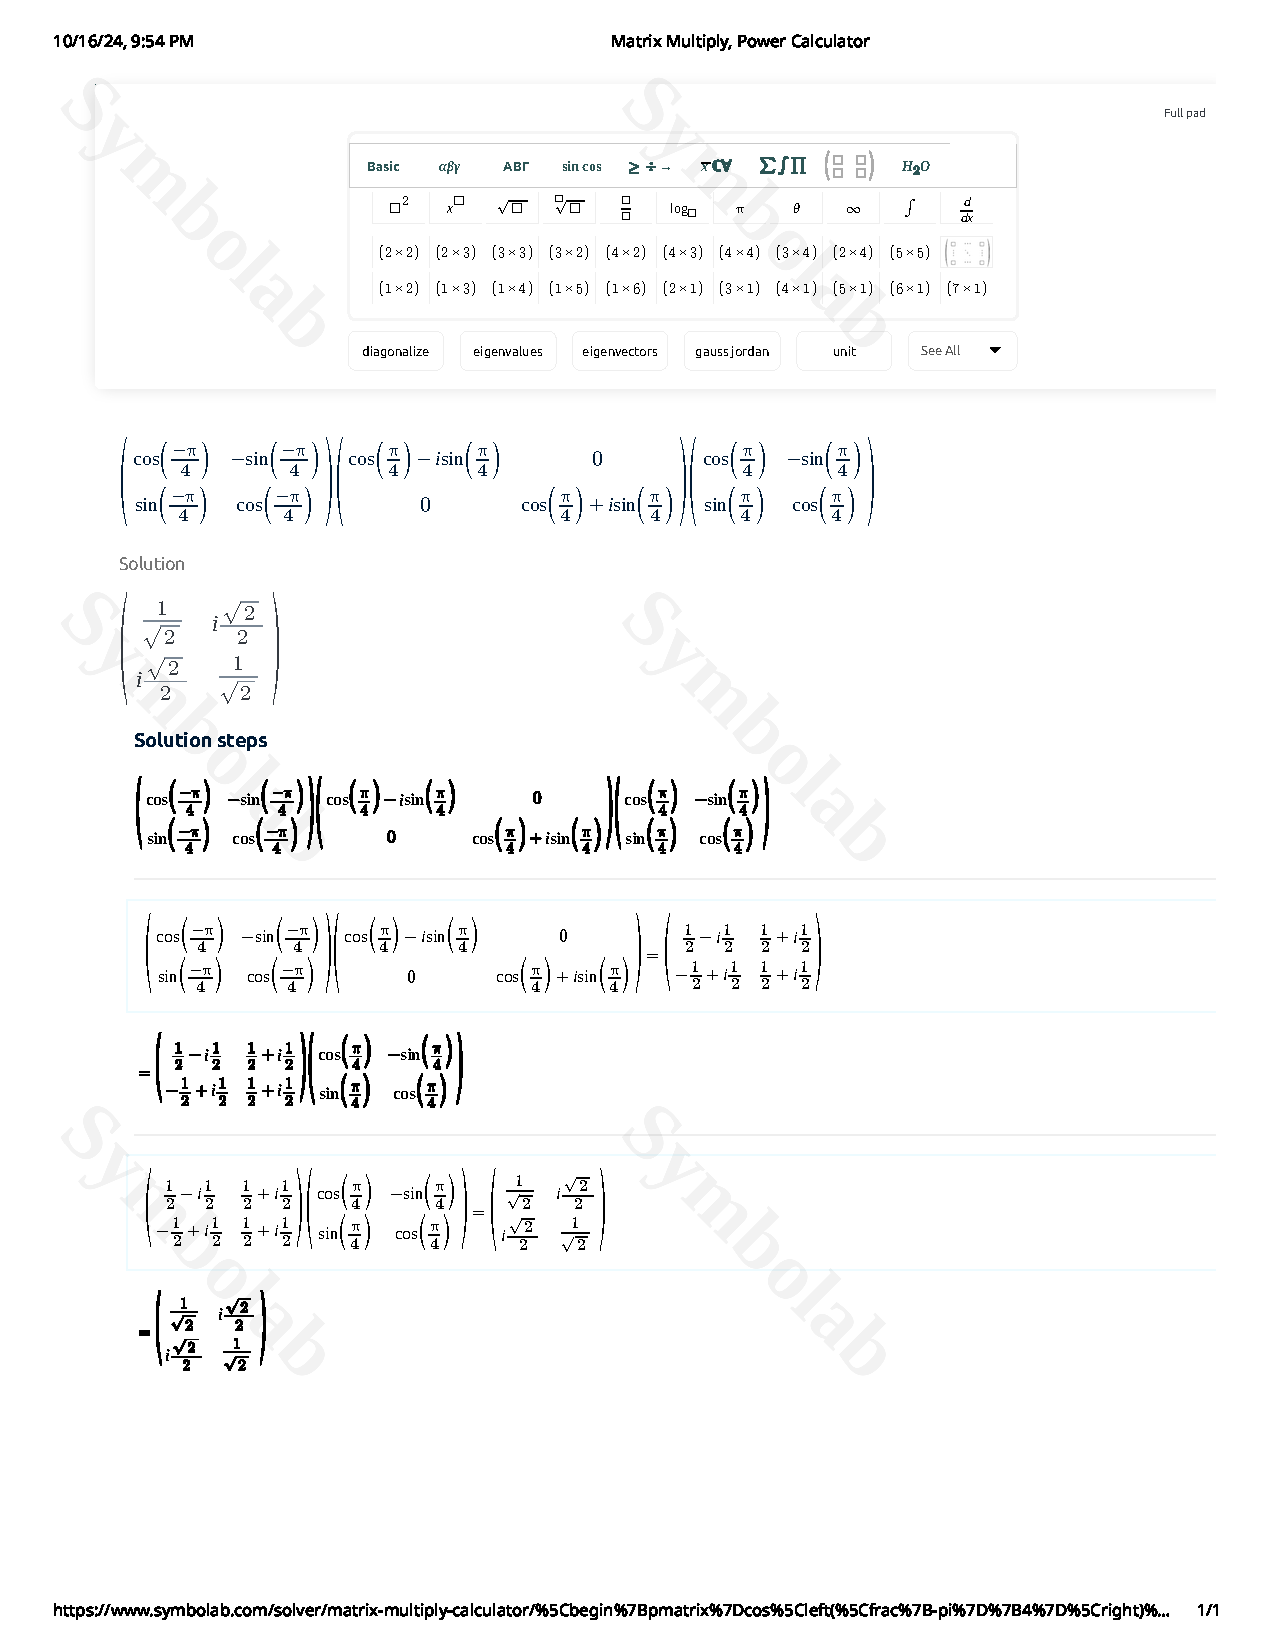
\includepdf{hw07-symbolab.pdf}
\newpage 
\subsection*{(b): insane place to type 300 additional lines of TiKZ code} 

This state is basically a \textbf{spinor} so I need to show a flagpole diagram to show what happens here. 

\begin{center}
% 3D AXIS with spherical coordinates
\tdplotsetmaincoords{60}{110}
\begin{tikzpicture}[scale=1.8,tdplot_main_coords]
  
  % VARIABLES
  \def\l{0.3} % length scale dark unit vector
  \def\rvec{1.2}
  \def\thetavec{0}
  \def\phivec{50}
  
  % AXES
  \coordinate (O) at (0,0,0);
  \tdplotsetcoord{P}{\rvec}{\thetavec}{\phivec}
  \draw[dashed,mydarkblue] (O)  -- (Pxy);
  \draw[thick,->] (0,0,0) -- (1,0,0) node[below left=-3]{$x$};
  \draw[thick,->] (0,0,0) -- (0,1,0) node[right=-1]{$y$};
  \draw[thick,->] (0,0,0) -- (0,0,1) node[anchor = south west]{$z$};
  \draw[unit vector] (0,0,0) -- (1.3*\l,0,0) node[above=3,left=-1,scale=0.8]{$\vu{x}$};
  \draw[unit vector] (0,0,0) -- (0,.9*\l,0) node[right=2,above=-1,scale=0.8]{$\vu{y}$};
  \draw[unit vector] (0,0,0) -- (0,0,\l) node[left,scale=0.8]{$\vu{z}$};
  
  % VECTORS
  \draw[dashed,mydarkblue] (P)  -- (Pxy);
  \draw[dashed,mydarkblue] (P)  -- (Pz);
  \draw[dashed,mydarkblue] (Py) -- (Pxy) -- (Px);
  \node[circle,inner sep=0.9,fill=myblue]
    (P') at ({\rvec*sin(\thetavec)*cos(\phivec)},{\rvec*sin(\thetavec)*sin(\phivec)},{\rvec*cos(\thetavec)}) {};
	\node[circle,inner sep=0.9,fill=myblue]
    (P'') at ({\rvec*sin(\thetavec)*cos(\phivec) + 0.3 },{\rvec*sin(\thetavec)*sin(\phivec)},{\rvec*cos(\thetavec)}) {};
  \draw[vector] (O)  -- (P') node[above right=-2] {P};
  \draw[vector] (P') -- (P''); 
  

\end{tikzpicture}
\tdplotsetmaincoords{60}{150}
\begin{tikzpicture}[scale=1.8,tdplot_main_coords]
  
  % VARIABLES
  \def\l{0.3} % length scale dark unit vector
  \def\rvec{1.2}
  \def\thetavec{90}
  \def\phivec{0}
  
  % AXES
  \coordinate (O) at (0,0,0);
  \tdplotsetcoord{P}{\rvec}{\thetavec}{\phivec}
  \draw[dashed,mydarkblue] (O)  -- (Pxy);
  \draw[thick,->] (0,0,0) -- (1,0,0) node[below left=-3]{$x$};
  \draw[thick,->] (0,0,0) -- (0,1,0) node[right=-1]{$y$};
  \draw[thick,->] (0,0,0) -- (0,0,1) node[above=-1]{$z$};
  \draw[unit vector] (0,0,0) -- (1.3*\l,0,0) node[above=3,left=-1,scale=0.8]{$\vu{x}$};
  \draw[unit vector] (0,0,0) -- (0,.9*\l,0) node[right=2,above=-1,scale=0.8]{$\vu{y}$};
  \draw[unit vector] (0,0,0) -- (0,0,\l) node[left,scale=0.8]{$\vu{z}$};
  
  % VECTORS
  \draw[dashed,mydarkblue] (P)  -- (Pxy);
  \draw[dashed,mydarkblue] (P)  -- (Pz);
  \draw[dashed,mydarkblue] (Py) -- (Pxy) -- (Px);
  \node[circle,inner sep=0.9,fill=myblue]
    (P') at ({\rvec*sin(\thetavec)*cos(\phivec)},{\rvec*sin(\thetavec)*sin(\phivec)},{\rvec*cos(\thetavec)}) {};
  \draw[vector] (O)  -- (P') node[above right=-2] {};
  
  % ARCS
  \tdplotsetthetaplanecoords{\phivec}
  \tdplotdrawarc[->,tdplot_rotated_coords]{(0,0,0)}{0.4}{0}{\thetavec}
    {right=2,above}{$\theta_1$}
	\draw[vector](P) -- (1.2,0,-0.3);
   
\end{tikzpicture}
\tdplotsetmaincoords{60}{150}
\begin{tikzpicture}[scale=1.8,tdplot_main_coords]
  
  % VARIABLES
  \def\l{0.3} % length scale dark unit vector
  \def\rvec{1.2}
  \def\thetavec{90}
  \def\phivec{90}
  
  % AXES
  \coordinate (O) at (0,0,0);
  \tdplotsetcoord{P}{\rvec}{\thetavec}{\phivec}
  \draw[dashed,mydarkblue] (O)  -- (Pxy);
  \draw[thick,->] (0,0,0) -- (1,0,0) node[below left=-3]{$x$};
  \draw[thick,->] (0,0,0) -- (0,1,0) node[right=-1]{$y$};
  \draw[thick,->] (0,0,0) -- (0,0,1) node[above=-1]{$z$};
  \draw[unit vector] (0,0,0) -- (1.3*\l,0,0) node[above=3,left=-1,scale=0.8]{$\vu{x}$};
  \draw[unit vector] (0,0,0) -- (0,.9*\l,0) node[right=2,above=-1,scale=0.8]{$\vu{y}$};
  \draw[unit vector] (0,0,0) -- (0,0,\l) node[left,scale=0.8]{$\vu{z}$};
  
  % VECTORS
  \draw[dashed,mydarkblue] (P)  -- (Pxy);
  \draw[dashed,mydarkblue] (P)  -- (Pz);
  \draw[dashed,mydarkblue] (Py) -- (Pxy) -- (Px);
  \node[circle,inner sep=0.9,fill=myblue]
    (P') at ({\rvec*sin(\thetavec)*cos(\phivec)},{\rvec*sin(\thetavec)*sin(\phivec)},{\rvec*cos(\thetavec)}) {};
  \draw[vector] (O)  -- (P') node[above right=-2] {};
  \draw[vector](P) -- (0,1.2,-0.3);
  % ARCS


	\tdplotsetthetaplanecoords{0}

\tdplotdrawarc[->,tdplot_rotated_coords]{(0,0,0)}{0.4}{0}{\thetavec}
    {right=2,above}{$\theta_1$}	

	\tdplotdrawarc{(0,0,0)}{0.4}{0}{\phivec}{anchor=north}{$\theta_2$}

  
\end{tikzpicture}
\tdplotsetmaincoords{60}{150}
\begin{tikzpicture}[scale=1.8,tdplot_main_coords]
  
  % VARIABLES
  \def\l{0.3} % length scale dark unit vector
  \def\rvec{1.2}
  \def\thetavec{90}
  \def\phivec{90}
  
  % AXES
  \coordinate (O) at (0,0,0);
  \tdplotsetcoord{P}{\rvec}{\thetavec}{\phivec}
  \draw[dashed,mydarkblue] (O)  -- (Pxy);
  \draw[thick,->] (0,0,0) -- (1,0,0) node[below left=-3]{$x$};
  \draw[thick,->] (0,0,0) -- (0,1,0) node[right=-1]{$y$};
  \draw[thick,->] (0,0,0) -- (0,0,1) node[above=-1]{$z$};
  \draw[unit vector] (0,0,0) -- (1.3*\l,0,0) node[above=3,left=-1,scale=0.8]{$\vu{x}$};
  \draw[unit vector] (0,0,0) -- (0,.9*\l,0) node[right=2,above=-1,scale=0.8]{$\vu{y}$};
  \draw[unit vector] (0,0,0) -- (0,0,\l) node[left,scale=0.8]{$\vu{z}$};
  
  % VECTORS
  \draw[dashed,mydarkblue] (P)  -- (Pxy);
  \draw[dashed,mydarkblue] (P)  -- (Pz);
  \draw[dashed,mydarkblue] (Py) -- (Pxy) -- (Px);
  \node[circle,inner sep=0.9,fill=myblue]
    (P') at ({\rvec*sin(\thetavec)*cos(\phivec)},{\rvec*sin(\thetavec)*sin(\phivec)},{\rvec*cos(\thetavec)}) {};
  \draw[vector] (O)  -- (P') node[above right=-2] {};
  \draw[vector](P) -- (-0.3,1.2,0);
  % ARCS


	\tdplotsetthetaplanecoords{0}

\tdplotdrawarc[->,tdplot_rotated_coords]{(0,0,0)}{0.4}{0}{\thetavec}
    {right=2,above}{$\theta_1$}	

	\tdplotdrawarc{(0,0,0)}{0.4}{0}{\phivec}{anchor=north}{$\theta_2$}

  
\end{tikzpicture}
\end{center}
The vector now lies along $\vec{y}$ which now validates the $\pi / 2$ angle difference. 

\begin{minipage}{0.5\textwidth}
	\[ 
	\vec{s} = 
	s \exp
	\left(
		- i \alpha / 2
	\right)
	\begin{bmatrix}
		\exp( - i \phi / 2 ) \cos(\theta / 2)
		\\
		\exp( i \phi / 2 ) \sin(\theta / 2)
	\end{bmatrix}
	\]
\end{minipage}
\begin{minipage}{0.5\textwidth}
\begin{figure}[H]
	\centering
	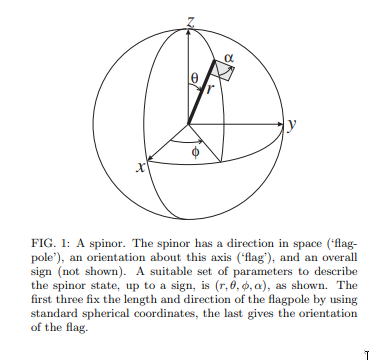
\includegraphics[width=\textwidth]{./ss/spinor-1.png}
\end{figure}
\end{minipage}
\newpage
\section*{Problem 4} 


\subsection*{(a)} 
The states as time progress is well understood which is 
\begin{align*}
	\ket{\psi_0} &:= \ket{m = 1}_z 
	\tag{$ t = 0 $} 
	\\
	\ket{\psi_1} &= \exp \left( - \frac{i}{\hb} \hat{H}_1 t\right) \ket{\psi_0} 
	\tag{$ 0 \le  t \le t_y $} 
	\\ 
	\ket{\psi_2} &= \exp 
	\left(- \frac{i}{\hb} \hat{H}_2 (t- t_y) \right)
	\exp \left( - \frac{i}{\hb} \hat{H}_1 t_y\right) \ket{\psi_0} 
	\tag{$t > t_y$ } 
	\\
\end{align*} 
The Hamiltonian is given by 
\begin{equation*}
\hat{H}(t) = 
\begin{cases}
	\hat{H}_1 = |\gamma| B_y \hat{S}_y & 0 < t < t_y \\ 
	\hat{H}_2 = |\gamma| B_z \hat{S}_z &t > t_y 
\end{cases}
\end{equation*} 
Crunch the computation of $\ket{\psi_1}$
\begin{align*}
	\ket{\psi_1(t_y)} &= 
	\exp \left( - \frac{i}{\hb} \hat{H}_1 t_y\right) \ket{\psi_0} 
	\\ 
	&= 
\exp 
\left(
- \frac{i}{\hb} | \gamma| B_y \hat{S}_y 
\left(
\frac{\pi }{2 | \gamma | B_y }
\right)
\right) 
\ket{\psi_0}
	\\ 
&= 
\exp
\left(
- \frac{i}{\hb} \hat{S}_y \frac{\pi}{2}\right) 
\ket{\psi_0}
\\
&= 
\hat R_y \left(\frac{\pi}{2} \right) \ket{\psi_0}
= 
\begin{pmatrix} 
\frac{1 + \cos (\pi / 2 ) }{2} \\ 
\frac{\sin ( \pi / 2)}{\sqrt{2} } \\ 
\frac{1 - \cos ( \pi / 2) }{2 }
\end{pmatrix} 
= \begin{pmatrix} \frac{1}{2} \\ \frac{1}{\sqrt{2} } \\ \frac{1}{2} \end{pmatrix}  
\tag{from previous problem solution} \end{align*}
Use this to finally find the required $\ket{\psi_2}$ and calling $\ket{\psi_1(t_y)} \equiv \ket{\psi_1}$
\begin{align*}
	\ket{\psi_2} &= 
\exp
\left(
- \frac{i}{\hb} \hat{H}_2 t + \frac{i}{\hb} \hat{H}_2 \frac{\pi }{2 |\gamma| B_y}
\right) \ket{\psi_1}
	\\
	&= 
\exp
\left(
- \frac{i}{\hb} |\gamma| B_z \hat{S}_z 
+ \frac{i}{\hb} |\gamma| B_z \hat{S}_z \frac{\pi }{2 | \gamma | B_y} 
\right) \ket{\psi_1}
	\\
	&= 
\exp
\left(
- \frac{i}{\hb} |\gamma| B_z \hat{S}_z 
+ \frac{i}{\hb} \frac{B_z}{B_y} \frac{\pi }{2} \hat{S}_z 
\right) \ket{\psi_1}
	\\
	&= 
\exp
\left( 
- \frac{i}{\hb} |\gamma| B_z \hat{S}_z  \right) \exp \left(
 \frac{i}{\hb} \frac{B_z}{B_y} \frac{\pi }{2} \hat{S}_z 
\right) \ket{\psi_1}
	\\
\end{align*}
The matrix $\hat{S}_z$ with some scalar $\Lambda ' = \Lambda / \hb$ so that it also get's rid of $\hb$ (for computational ease), and I don't really make much distinction from $\Lambda, \Lambda'$, so you can imagine that $ \hb \Lambda \implies \Lambda$ where planks constant is sucked into the $\Lambda$ and we will take care of it at the end by pulling it out.  
\begin{align*}
	\hat{S}_z &= \hb 
	\begin{bmatrix} 1 & 0 & 0 \\ 0 & 0 & 0 \\ 0 & 0 & -1 \end{bmatrix} \\
	\Lambda \hat{S}_z &= 
	\begin{bmatrix} \hb \Lambda & 0 & 0 \\ 0 & 0 & 0 \\ 0 & 0 & -\hb \Lambda \end{bmatrix} 
	\underbrace{\implies}_{\text{suck $\hb$ into  $\Lambda $}} 
	\begin{bmatrix} \Lambda & 0 & 0 \\ 0 & 0 & 0 \\ 0 & 0 & - \Lambda \end{bmatrix} 
	\\
	\mathrm{e}^{ i \Lambda \hat{S}_z} = 
	\exp(  i \Lambda \hat{S}_z ) &= 
\hat{I} + i \frac{\Lambda \hat{S}_z}{1 !}  + 
i ^2 \frac{\Lambda ^2 \hat{S}_z ^2}{2!} + 
i ^3\frac{\Lambda^3 \hat{S}_z ^3}{3!} + 
i ^{4}\frac{\Lambda^4 \hat{S}_z ^4}{4!} + 
\cdots 
	\\
	&= 
\hat{I} + 
\Lambda 
	\begin{bmatrix} i&0&0\\0&0&0\\0&0&-i \end{bmatrix} 
	- 
	\frac{\Lambda^2}{2!}
	\begin{bmatrix} 1&0&0\\0&0&0\\0&0&1 \end{bmatrix} 
	-
	\frac{\Lambda^3}{3!}
	\begin{bmatrix} i&0&0\\0&0&0\\0&0&-i \end{bmatrix} 
	+ 
\frac{\Lambda^{4}}{4!}
	\begin{bmatrix} 1&0&0\\0&0&0\\0&0&1 \end{bmatrix}  
	+ \cdots
	\\
	&=  
\hat{I} 
	- 
	\frac{\Lambda^2}{2!}
	\begin{bmatrix} 1&0&0\\0&0&0\\0&0&1 \end{bmatrix}  
+ \frac{\Lambda^{4}}{4!}
	\begin{bmatrix} 1&0&0\\0&0&0\\0&0&1 \end{bmatrix}  
	+ 
	\cdots 
	+
	i 
	\left(
\Lambda 
	\begin{bmatrix} 1&0&0\\0&0&0\\0&0&-1 \end{bmatrix} 
	-
	\frac{\Lambda^3}{3!}
	\begin{bmatrix} 1&0&0\\0&0&0\\0&0&-1 \end{bmatrix} 
+ \cdots
		\right) 
\\ 
			 &= 
			\hat{I} 
			\textcolor{blue}{		-
	\begin{bmatrix} 1&0&0\\0&0&0\\0&0&1 \end{bmatrix}  
+
\begin{bmatrix} 1&0&0\\0&0&0\\0&0&1 \end{bmatrix}   } 
	-
	\frac{\Lambda^2}{2!}
	\begin{bmatrix} 1&0&0\\0&0&0\\0&0&1 \end{bmatrix}  
+ \frac{\Lambda^{4}}{4!}
	\begin{bmatrix} 1&0&0\\0&0&0\\0&0&1 \end{bmatrix}  
	+ 
	\cdots 
		      \\ & 	\textcolor{blue}{+ \cdots +}  
	i 
	\left(
\Lambda 
	\begin{bmatrix} 1&0&0\\0&0&0\\0&0&-1 \end{bmatrix} 
	-
	\frac{\Lambda^3}{3!}
	\begin{bmatrix} 1&0&0\\0&0&0\\0&0&-1 \end{bmatrix} 
+ \cdots
		\right) \\
			 &= 
			\left(\hat{I} 
			-
	\begin{bmatrix} 1&0&0\\0&0&0\\0&0&1 \end{bmatrix}  \right)
+
\left(	1 -
	\frac{\Lambda^2}{2!}
+ \frac{\Lambda^{4}}{4!}
	+ 
	\cdots \right)
	\begin{bmatrix} 1&0&0\\0&0&0\\0&0&1 \end{bmatrix}   
		+
	i 
	\left(
\Lambda 
	-
	\frac{\Lambda^3}{3!}
+ \cdots
		\right) 
	\begin{bmatrix} 1&0&0\\0&0&0\\0&0&-1 \end{bmatrix} 
	\\ &= 
	\left(\begin{bmatrix} 1&0&0\\0&1&0\\0&0&1 \end{bmatrix} -
	\begin{bmatrix} 1&0&0\\0&0&0\\0&0&1 \end{bmatrix}   \right)
	+  
	\begin{bmatrix} \cos \Lambda & 0 & 0 \\ 
	0 & 0 & 0 \\ 
0 & 0 & \cos \Lambda \end{bmatrix} 
+ 
		\begin{bmatrix} i \sin \Lambda & 0 & 0 
		\\ 0 & 0 & 0 \\ 
	0 & 0 & - i \sin \Lambda
\end{bmatrix} 
	\\
	&= 
			\begin{bmatrix} \cos \Lambda + i \sin \Lambda &0&0\\
			0&1&0\\
		0&0& \cos \Lambda - i \sin \Lambda \end{bmatrix} 
	\\
	&= 
			\begin{bmatrix} 
				\exp 
			\left(  i \Lambda \right )
			&0&0\\
			0&1&0\\
		0&0& 
				\exp 
			\left(- i \Lambda \right)  \end{bmatrix} 
			\underbrace{\implies}_{\text{push $\hb$ out}}
			\begin{bmatrix} 
				\exp 
			\left(  i \hb \Lambda \right )
			&0&0\\
			0&1&0\\
		0&0& 
				\exp 
			\left(- i \hb \Lambda \right)  \end{bmatrix} 
\end{align*}





\begin{align*}
& \exp
\left( 
- \frac{i}{\hb} |\gamma| B_z \hat{S}_z t  \right) \exp \left(
 \frac{i}{\hb} \frac{B_z}{B_y} \frac{\pi }{2} \hat{S}_z 
\right) \ket{\psi_1}  \\ 
&= 
\begin{bmatrix} 
\exp 
\left(  -i |\gamma| B_z  t\right )
&0&0\\
0&1&0\\
0&0& 
\exp 
\left(i |\gamma| B_z t  \right)  \end{bmatrix} 
\begin{bmatrix} 
\exp 
\left(  i \frac{B_z}{B_y} \frac{\pi}{2} \right )
&0&0\\
0&1&0\\
0&0& 
\exp 
\left( - i \frac{B_z}{B_y} \frac{\pi}{2} \right )
 \end{bmatrix} 
\begin{pmatrix} 
	1 / 2 \\
	1 / \sqrt{2}  \\ 
	1 / 2 
\end{pmatrix}\\  
&= 
\begin{bmatrix} 
\exp 
\left(  -i |\gamma| B_z  t\right )
&0&0\\
0&1&0\\
0&0& 
\exp 
\left(i |\gamma| B_z t  \right)  \end{bmatrix} 
\begin{bmatrix} 
	(1 / 2 )\exp 
\left(  i \frac{B_z}{B_y} \frac{\pi}{2} \right )
\\
1 / \sqrt{2} \\
(1 / 2 )\exp 
\left( - i \frac{B_z}{B_y} \frac{\pi}{2} \right )
 \end{bmatrix}\\ 
 &= 
\begin{bmatrix} 
	(1 / 2 )\exp 
\left(  i \frac{B_z}{B_y} \frac{\pi}{2} - i | \gamma | B_z t \right )
\\
1 / \sqrt{2} \\
(1 / 2 )\exp 
\left( - i \frac{B_z}{B_y} \frac{\pi}{2} + i | \gamma | B_z t\right )
 \end{bmatrix}\\ 
\end{align*}
So after all these algebraic and matrix warfare 
\[
\ket{\psi_2(t)} = 
\begin{bmatrix} 
	(1 / 2 )\exp 
\left(  i \frac{B_z}{B_y} \frac{\pi}{2} - i | \gamma | B_z t \right )
\\
1 / \sqrt{2} \\
(1 / 2 )\exp 
\left( - i \frac{B_z}{B_y} \frac{\pi}{2} + i | \gamma | B_z t\right )
 \end{bmatrix} \equiv 
 \begin{bmatrix} (1 / 2) \exp( - i \theta) \\ 1 / \sqrt{2}  \\ (1 / 2) \exp( i \theta) \end{bmatrix} = 
 \begin{bmatrix} \frac{1}{2} e^{- i \theta} \\ \frac{1}{\sqrt{2} } \\ \frac{1}{2}e^{i \theta} \end{bmatrix} 
\] 

\subsection*{(b)} 
For any desired state $\ket{\Psi}$ the probability of getting that 
\[
\braket{ \psi_2(t) | \Psi | } ^2 \implies \braket{\Psi | \psi_2(t)}
\braket{\psi_2(t) | \Psi} \] 
The desired state this case 
\[
	\hat{S}_z \ket{m = 1}_z = \hb \ket{m=1}_z  \implies \ket{m = 1}_z = \ket{\Psi} = \begin{pmatrix} 1 \\ 0 \\ 0 \end{pmatrix} 
\] 
\begin{align*}
	\braket{\psi_2(t) | \Psi} ^2 &= 
	\left(
	\begin{bmatrix} 1&0&0 \end{bmatrix} 
 \begin{bmatrix} \frac{1}{2} e^{- i \theta} \\ \frac{1}{\sqrt{2} } \\ \frac{1}{2}e^{i \theta} \end{bmatrix} 
	\right)
	\left(
	\begin{bmatrix} \frac{1}{2} e^{ i \theta} & \frac{1}{\sqrt{2} } & \frac{1}{2}e^{- i \theta} \end{bmatrix} 
	\begin{bmatrix} 1\\0\\0 \end{bmatrix} 
	\right) = \frac{1}{4}
\end{align*}
\subsection*{(c)} 
\begin{align*}
	\hat{S}_z \ket{m=0}_z = \ket{0} \implies  \ket{\Psi} = \begin{pmatrix} 0\\1\\0 \end{pmatrix} 
\end{align*}
\begin{align*}
	\braket{\psi_2(t) | \Psi} ^2 &= 
	\left(
	\begin{bmatrix} 0&1&0 \end{bmatrix} 
 \begin{bmatrix} \frac{1}{2} e^{- i \theta} \\ \frac{1}{\sqrt{2} } \\ \frac{1}{2}e^{i \theta} \end{bmatrix} 
	\right)
	\left(
	\begin{bmatrix} \frac{1}{2} e^{ i \theta} & \frac{1}{\sqrt{2} } & \frac{1}{2}e^{- i \theta} \end{bmatrix} 
	\begin{bmatrix} 0\\1\\0 \end{bmatrix} 
	\right) = \frac{1}{2}
\end{align*}

\subsection*{(d)} 
\begin{align*}
	\hat{S}_x \ket{m = 0}_x = \ket{0} \implies 
	\begin{bmatrix} 
	0& \hb / \sqrt{2}  &  0 \\ 
\hb / \sqrt{2}  & 0 & \hb / \sqrt{2}  \\ 
0 & \hb / \sqrt{2}  & 0
\end{bmatrix} 
\begin{bmatrix} x_1 \\ x_2 \\ x_3 \end{bmatrix}  = 
\begin{bmatrix} m_2 \\ m_1 + m_3 \\ m_2 \end{bmatrix} = 
\begin{bmatrix} 0\\0\\0 \end{bmatrix} 
\implies 
\ket{m = 0}_x= \ket{\Psi} = \frac{1}{\sqrt{2} } \begin{bmatrix} 1\\0\\-1 \end{bmatrix} 
\end{align*}
\begin{align*}
	\braket{\psi_2(t) | \Psi} ^2 &= 
	\frac{1}{2} 
	\left(
	\begin{bmatrix} 1&0&-1 \end{bmatrix} 
 \begin{bmatrix} \frac{1}{2} e^{- i \theta} \\ \frac{1}{\sqrt{2} } \\ \frac{1}{2}e^{i \theta} \end{bmatrix} 
	\right)
	\left(
	\begin{bmatrix} \frac{1}{2} e^{ i \theta} & \frac{1}{\sqrt{2} } & \frac{1}{2}e^{- i \theta} \end{bmatrix} 
	\begin{bmatrix} 1\\0\\-1 \end{bmatrix} 
	\right) \\
	&= 
\frac{1}{2}
\left[
	\left(\frac{1}{2}e^{-i \theta} - \frac{1}{2} e^{i \theta}\right)
	\left(\frac{1}{2}e^{i \theta} - \frac{1}{2}e^{- i \theta}\right)
\right]
	\\
	&= -
\frac{1}{2}
\left[
	\left(\frac{1}{2}e^{-i \theta} - \frac{1}{2} e^{i \theta}\right)
	\left(\frac{1}{2}e^{-i \theta} - \frac{1}{2}e^{ i \theta}\right)
\right]
	\\
	&= -
\frac{1}{2}
	\left(\frac{1}{2}e^{-i \theta} - \frac{1}{2} e^{i \theta}\right)^2
	\\
	&= 
- \frac{1}{8} 
\left(e^{- 2 i \theta} + e^{2 i \theta} - 2 e^{-i \theta} e^{ i \theta}\right)
	\\
	&= 
	\frac{1}{8} 
	\left(
2 - e^{- 2 i \theta} - e^{ 2 i \theta}
	\right)
	\\
	&= 
\frac{1 - \frac{e^{- 2 i \theta } + e^{ 2 i \theta} }{2} }{4}
	\\ 
	&= 
\frac{1 - \cos(2 \theta )}{4}
	\\ 
	&= \frac{1}{2}
\frac{1 - \cos(2 \theta )}{2}
	\\ 
	&= \frac{1}{2}
	\sin ^2 \theta 
	\\ 
	&= \frac{1}{2}
\sin^2 \left(
|\gamma| B_z t - \frac{\pi}{2} \frac{B_z}{B_y}
\right)
	\\
\end{align*}
 \[
	 \mathcal P _{(S_x = 0) }
	= \frac{1}{2}
\sin^2 \left(
|\gamma| B_z t - \frac{\pi}{2} \frac{B_z}{B_y}
\right)
 \] 

	\newpage
\section*{Problem 5} 
\subsection*{(a)}
To resist my sanity from leaving my head i am going to make some changes on the notation so 
\[
	\varepsilon_{kij} \varepsilon_{kmn} = \delta_{im} \delta _{jn} - \delta_{in} \delta_{jm} 
\] 
\begin{align*}
	\vec{A} \times (\vec{B} \times  \vec{C}) 
	&= [\varepsilon_{ijk} a_j (\varepsilon_{kmn} b_m c_n) ]_i \\ 
	&= [\varepsilon_{kij} a_j (\varepsilon_{kmn} b_m c_n) ]_i \\ 
	&= [\varepsilon_{kij} \varepsilon_{kmn} a_j b_m c_n ]_i \\ 
	&= [(\delta_{im} \delta_{jn} - \delta_{in} \delta_{jm} ) a_j b_m c_n ]_i \\ 
	&= [\delta_{im} \delta_{jn} a_j b_m c_n - \delta_{in} \delta_{jm}  a_j b_m c_n ]_i \\ 
	&= [\delta_{im} (\delta_{jn} a_j c_n) b_m  - \delta_{in} (\delta_{jm} a_j b_m) c_n ]_i \\ 
	&= [ (a_j c_j) b_i  - (a_j b_j) c_i ]_i \\  
	&= [ (\vec{A} \cdot \vec{C} ) b_i - (\vec{A} \cdot \vec{B}) c_i ] _i \\
	&= \vec{B} \left(\vec{A} \cdot \vec{C}\right) - \vec{C} \left(\vec{A} \cdot \vec{B}\right) \tag{taking sum over all component} \\ 
\end{align*}
\subsection*{(b)} 

\begin{align*} 
	\frac{\mathrm{d} }{\mathrm{d} t}\left(
	\vec{\mu} \cdot \vec{\mu}
	\right) = 
	2 {\vec{\mu}} \cdot  \frac{\mathrm{d} \vec{\mu}}{\mathrm{d} t} 
	&= 2 \vec{\mu} \cdot  \left(\gamma \vec{\mu} \times \vec{B}(t) \right)  \\ 
	&= 
	0 \tag{$\vec{\mu} \perp \gamma \vec{\mu} \times \vec{B}(t)$ }
	\\
	& \implies 
	\vec{\mu} (t) \cdot  \vec{\mu} (t) = \text{const}
\end{align*}


\subsection*{(c)}
Solve for the magnetic field first in terms of $\vec{n}$ 
\begin{align*}
	\vec{B}(t) &= \vec{B}_1 (t) + \vec{B}_2 (t) \\ 
	&= B_1(t) \vec{n}(t) + \left( - \frac{1}{\gamma} \vec{n} (t)\times \frac{\mathrm{d} }{\mathrm{d} t} \vec{n} (t)\right)
\end{align*}

We compute the rate of change of $\vec{\mu}$ and then dot product $\vec{n}$ with it to get the required solution
\begin{align*}
\frac{\mathrm{d} \vec{\mu}}{\mathrm{d} t} = \gamma \vec{\mu} \times  \vec{B} &= 
\gamma B_1(t) (\vec{\mu} \times \vec{n}) +
\vec{\mu} \times  
\left(- \vec{n} \times  \frac{\mathrm{d} }{\mathrm{d} t} \vec{n}\right)
\\ 
&= 
\gamma B_1(t) (\vec{\mu} \times \vec{n}) -
\vec{\mu} \times  
\left( \vec{n} \times  \frac{\mathrm{d} }{\mathrm{d} t} \vec{n}\right)
\\ 
&= 
\gamma B_1(t) (\vec{\mu} \times \vec{n}) 
- 
\left(
\vec{n} 
\left(\vec{\mu} \cdot  \frac{\mathrm{d}\vec{n} }{\mathrm{d} t} \right)
- 
\frac{\mathrm{d}\vec{n} }{\mathrm{d} t} 
\left(
	\vec{\mu} \cdot \vec{n}
\right)
\right)
\end{align*}
Now dotting $\vec{n}$ with both sides 
\begin{align*}
\vec{n} \cdot  
\frac{\mathrm{d} \vec{\mu}}{\mathrm{d} t} &= 
0 - 
\left(
\vec{n} \cdot  \vec{n} 
\left(\vec{\mu} \cdot  \frac{\mathrm{d} \vec{n}}{\mathrm{d} t}\right)
- 
\vec{n} \cdot  \frac{\mathrm{d} \vec{n}}{\mathrm{d} t} \left(\vec{\mu} \cdot  \vec{n}\right)
\right) 
\tag{$\vec{n} \perp \vec{\mu} \times  \vec{n} $ } 
\\ 
\vec{n} \cdot  
\frac{\mathrm{d} \vec{\mu}}{\mathrm{d} t} &= 
 - 
\left(\vec{\mu} \cdot  \frac{\mathrm{d} \vec{n}}{\mathrm{d} t}\right)
+ 
\vec{n} \cdot  \frac{\mathrm{d} \vec{n}}{\mathrm{d} t} \left(\vec{\mu} \cdot  \vec{n}\right) 
\tag{$\vec{n} \cdot  \vec{n} = 1$}
\\ 
\vec{n} \cdot  
\frac{\mathrm{d} \vec{\mu}}{\mathrm{d} t} &= 
 - 
\left(\vec{\mu} \cdot  \frac{\mathrm{d} \vec{n}}{\mathrm{d} t}\right)
+0   
\tag{$\vec{n} \cdot \frac{\mathrm{d} \vec{n}}{\mathrm{d} t} = 0$ as $\vec{n} \cdot  \vec{n} = 0$}
\\ 
\vec{n} \cdot  
\frac{\mathrm{d} \vec{\mu}}{\mathrm{d} t} &= 
 - 
\vec{\mu} \cdot  \frac{\mathrm{d} \vec{n}}{\mathrm{d} t}
\end{align*} 
Now solving for the $\vec{n} \cdot \vec{\mu}$ derivative 
\begin{align*} 
	\implies 
\frac{\mathrm{d} }{\mathrm{d} t} \left(
\vec{n}(t) \cdot  \vec{\mu}(t) 
	\right) &= 
\vec{\mu}(t) \frac{\mathrm{d} \vec{n}(t)}{\mathrm{d} t} + 
\vec{n}(t) \frac{\mathrm{d} \vec{\mu}(t)}{\mathrm{d} t} = 0
\end{align*}
Hence approving $\vec{n} \cdot \vec{\mu}$ is a constant. 












\newpage 
\section*{appendix: unnecessary things only for aesthetic purposes}
\subsection*{The TiKZ figure}
\begin{center}
	% 3D AXIS with spherical coordinates
	\tdplotsetmaincoords{60}{110}
	\begin{tikzpicture}[scale=1.8,tdplot_main_coords]
	  
	  % VARIABLES
	  \def\l{0.3} % length scale dark unit vector
	  \def\rvec{1.2}
	  \def\thetavec{0}
	  \def\phivec{50}
	  
	  % AXES
	  \coordinate (O) at (0,0,0);
	  \tdplotsetcoord{P}{\rvec}{\thetavec}{\phivec}
	  \draw[dashed,mydarkblue] (O)  -- (Pxy);
	  \draw[thick,->] (0,0,0) -- (1,0,0) node[below left=-3]{$x$};
	  \draw[thick,->] (0,0,0) -- (0,1,0) node[right=-1]{$y$};
	  \draw[thick,->] (0,0,0) -- (0,0,1) node[anchor = south west]{$z$};
	  \draw[unit vector] (0,0,0) -- (1.3*\l,0,0) node[above=3,left=-1,scale=0.8]{$\vu{x}$};
	  \draw[unit vector] (0,0,0) -- (0,.9*\l,0) node[right=2,above=-1,scale=0.8]{$\vu{y}$};
	  \draw[unit vector] (0,0,0) -- (0,0,\l) node[left,scale=0.8]{$\vu{z}$};
	  
	  % VECTORS
	  \draw[dashed,mydarkblue] (P)  -- (Pxy);
	  \draw[dashed,mydarkblue] (P)  -- (Pz);
	  \draw[dashed,mydarkblue] (Py) -- (Pxy) -- (Px);
	  \node[circle,inner sep=0.9,fill=myblue]
		(P') at ({\rvec*sin(\thetavec)*cos(\phivec)},{\rvec*sin(\thetavec)*sin(\phivec)},{\rvec*cos(\thetavec)}) {};
		\node[circle,inner sep=0.9,fill=myblue]
		(P'') at ({\rvec*sin(\thetavec)*cos(\phivec) + 0.3 },{\rvec*sin(\thetavec)*sin(\phivec)},{\rvec*cos(\thetavec)}) {};
	  \draw[vector] (O)  -- (P') node[above right=-2] {P};
	  \draw[vector] (P') -- (P''); 
	  
	
	\end{tikzpicture}
	\tdplotsetmaincoords{60}{150}
	\begin{tikzpicture}[scale=1.8,tdplot_main_coords]
	  
	  % VARIABLES
	  \def\l{0.3} % length scale dark unit vector
	  \def\rvec{1.2}
	  \def\thetavec{90}
	  \def\phivec{0}
	  
	  % AXES
	  \coordinate (O) at (0,0,0);
	  \tdplotsetcoord{P}{\rvec}{\thetavec}{\phivec}
	  \draw[dashed,mydarkblue] (O)  -- (Pxy);
	  \draw[thick,->] (0,0,0) -- (1,0,0) node[below left=-3]{$x$};
	  \draw[thick,->] (0,0,0) -- (0,1,0) node[right=-1]{$y$};
	  \draw[thick,->] (0,0,0) -- (0,0,1) node[above=-1]{$z$};
	  \draw[unit vector] (0,0,0) -- (1.3*\l,0,0) node[above=3,left=-1,scale=0.8]{$\vu{x}$};
	  \draw[unit vector] (0,0,0) -- (0,.9*\l,0) node[right=2,above=-1,scale=0.8]{$\vu{y}$};
	  \draw[unit vector] (0,0,0) -- (0,0,\l) node[left,scale=0.8]{$\vu{z}$};
	  
	  % VECTORS
	  \draw[dashed,mydarkblue] (P)  -- (Pxy);
	  \draw[dashed,mydarkblue] (P)  -- (Pz);
	  \draw[dashed,mydarkblue] (Py) -- (Pxy) -- (Px);
	  \node[circle,inner sep=0.9,fill=myblue]
		(P') at ({\rvec*sin(\thetavec)*cos(\phivec)},{\rvec*sin(\thetavec)*sin(\phivec)},{\rvec*cos(\thetavec)}) {};
	  \draw[vector] (O)  -- (P') node[above right=-2] {};
	  
	  % ARCS
	  \tdplotsetthetaplanecoords{\phivec}
	  \tdplotdrawarc[->,tdplot_rotated_coords]{(0,0,0)}{0.4}{0}{\thetavec}
		{right=2,above}{$\theta_1$}
		\draw[vector](P) -- (1.2,0,-0.3);
	   
	\end{tikzpicture}
	\tdplotsetmaincoords{60}{150}
	\begin{tikzpicture}[scale=1.8,tdplot_main_coords]
	  
	  % VARIABLES
	  \def\l{0.3} % length scale dark unit vector
	  \def\rvec{1.2}
	  \def\thetavec{90}
	  \def\phivec{90}
	  
	  % AXES
	  \coordinate (O) at (0,0,0);
	  \tdplotsetcoord{P}{\rvec}{\thetavec}{\phivec}
	  \draw[dashed,mydarkblue] (O)  -- (Pxy);
	  \draw[thick,->] (0,0,0) -- (1,0,0) node[below left=-3]{$x$};
	  \draw[thick,->] (0,0,0) -- (0,1,0) node[right=-1]{$y$};
	  \draw[thick,->] (0,0,0) -- (0,0,1) node[above=-1]{$z$};
	  \draw[unit vector] (0,0,0) -- (1.3*\l,0,0) node[above=3,left=-1,scale=0.8]{$\vu{x}$};
	  \draw[unit vector] (0,0,0) -- (0,.9*\l,0) node[right=2,above=-1,scale=0.8]{$\vu{y}$};
	  \draw[unit vector] (0,0,0) -- (0,0,\l) node[left,scale=0.8]{$\vu{z}$};
	  
	  % VECTORS
	  \draw[dashed,mydarkblue] (P)  -- (Pxy);
	  \draw[dashed,mydarkblue] (P)  -- (Pz);
	  \draw[dashed,mydarkblue] (Py) -- (Pxy) -- (Px);
	  \node[circle,inner sep=0.9,fill=myblue]
		(P') at ({\rvec*sin(\thetavec)*cos(\phivec)},{\rvec*sin(\thetavec)*sin(\phivec)},{\rvec*cos(\thetavec)}) {};
	  \draw[vector] (O)  -- (P') node[above right=-2] {};
	  \draw[vector](P) -- (0,1.2,-0.3);
	  % ARCS
	
	
		\tdplotsetthetaplanecoords{0}
	
	\tdplotdrawarc[->,tdplot_rotated_coords]{(0,0,0)}{0.4}{0}{\thetavec}
		{right=2,above}{$\theta_1$}	
	
		\tdplotdrawarc{(0,0,0)}{0.4}{0}{\phivec}{anchor=north}{$\theta_2$}
	
	  
	\end{tikzpicture}
	\tdplotsetmaincoords{60}{130}
	\begin{tikzpicture}[scale=1.8,tdplot_main_coords]
	  
	  % VARIABLES
	  \def\l{0.3} % length scale dark unit vector
	  \def\rvec{1.2}
	  \def\thetavec{0}
	  \def\phivec{50}
	  
	  % AXES
	  \coordinate (O) at (0,0,0);
	  \tdplotsetcoord{P}{\rvec}{\thetavec}{\phivec}
	  \draw[dashed,mydarkblue] (O)  -- (Pxy);
	  \draw[thick,->] (0,0,0) -- (1,0,0) node[below left=-3]{$x$};
	  \draw[thick,->] (0,0,0) -- (0,1,0) node[right=-1]{$y$};
	  \draw[thick,->] (0,0,0) -- (0,0,1) node[anchor = north west]{$z$};
	
	  
	  % VECTORS
	  \draw[dashed,mydarkblue] (P)  -- (Pxy);
	  \draw[dashed,mydarkblue] (P)  -- (Pz);
	  \draw[dashed,mydarkblue] (Py) -- (Pxy) -- (Px);
	  \node[circle,inner sep=0.9,fill=myblue]
		(P') at ({\rvec*sin(\thetavec)*cos(\phivec)},{\rvec*sin(\thetavec)*sin(\phivec)},{\rvec*cos(\thetavec)}) {};
	  \draw[vector] (O)  -- (P') node[above right=-2] {};
	  \draw[dotted, vector](P) -- (0.3,0,1.2);
	  \draw[vector](P) -- (0,0.3,1.2);
	  
	  % ARCS
	
	
	  \tdplotdrawarc{(0,0,0)}{0.4}{90}{0}{anchor=north}{$\theta_1$}
	  \tdplotsetrotatedcoords{-90}{-90}{0}
	  \tdplotdrawarc[tdplot_rotated_coords]{(0,0,0)}{0.4}{90}{0}{anchor=south}{$\theta_2$}
	  \tdplotsetrotatedcoords{0}{-90}{0}
	  \tdplotdrawarc[tdplot_rotated_coords]{(0,0,0)}{0.4}{90}{0}{anchor=south}{$\theta_3$}
	
	  
	\end{tikzpicture}
	\end{center}

	\begin{multicols}{2}
\begin{tiny}\begin{verbatim}
	\begin{center}
		% 3D AXIS with spherical coordinates
		\tdplotsetmaincoords{60}{110}
		\begin{tikzpicture}[scale=1.8,tdplot_main_coords]
		  
		  % VARIABLES
		  \def\l{0.3} % length scale dark unit vector
		  \def\rvec{1.2}
		  \def\thetavec{0}
		  \def\phivec{50}
		  
		  % AXES
		  \coordinate (O) at (0,0,0);
		  \tdplotsetcoord{P}{\rvec}{\thetavec}{\phivec}
		  \draw[dashed,mydarkblue] (O)  -- (Pxy);
		  \draw[thick,->] (0,0,0) -- (1,0,0) node[below left=-3]{$x$};
		  \draw[thick,->] (0,0,0) -- (0,1,0) node[right=-1]{$y$};
		  \draw[thick,->] (0,0,0) -- (0,0,1) node[anchor = south west]{$z$};
		  \draw[unit vector] (0,0,0) -- (1.3*\l,0,0) node[above=3,left=-1,scale=0.8]{$\vu{x}$};
		  \draw[unit vector] (0,0,0) -- (0,.9*\l,0) node[right=2,above=-1,scale=0.8]{$\vu{y}$};
		  \draw[unit vector] (0,0,0) -- (0,0,\l) node[left,scale=0.8]{$\vu{z}$};
		  
		  % VECTORS
		  \draw[dashed,mydarkblue] (P)  -- (Pxy);
		  \draw[dashed,mydarkblue] (P)  -- (Pz);
		  \draw[dashed,mydarkblue] (Py) -- (Pxy) -- (Px);
		  \node[circle,inner sep=0.9,fill=myblue]
			(P') at ({\rvec*sin(\thetavec)*cos(\phivec)},{\rvec*sin(\thetavec)*sin(\phivec)},
			{\rvec*cos(\thetavec)}) {};
			\node[circle,inner sep=0.9,fill=myblue]
			(P'') at ({\rvec*sin(\thetavec)*cos(\phivec) + 0.3 },{\rvec*sin(\thetavec)*sin(\phivec)},
			{\rvec*cos(\thetavec)}) {};
		  \draw[vector] (O)  -- (P') node[above right=-2] {P};
		  \draw[vector] (P') -- (P''); 
		  
		
		\end{tikzpicture}
		\tdplotsetmaincoords{60}{150}
		\begin{tikzpicture}[scale=1.8,tdplot_main_coords]
		  
		  % VARIABLES
		  \def\l{0.3} % length scale dark unit vector
		  \def\rvec{1.2}
		  \def\thetavec{90}
		  \def\phivec{0}
		  
		  % AXES
		  \coordinate (O) at (0,0,0);
		  \tdplotsetcoord{P}{\rvec}{\thetavec}{\phivec}
		  \draw[dashed,mydarkblue] (O)  -- (Pxy);
		  \draw[thick,->] (0,0,0) -- (1,0,0) node[below left=-3]{$x$};
		  \draw[thick,->] (0,0,0) -- (0,1,0) node[right=-1]{$y$};
		  \draw[thick,->] (0,0,0) -- (0,0,1) node[above=-1]{$z$};
		  \draw[unit vector] (0,0,0) -- (1.3*\l,0,0) node[above=3,left=-1,scale=0.8]{$\vu{x}$};
		  \draw[unit vector] (0,0,0) -- (0,.9*\l,0) node[right=2,above=-1,scale=0.8]{$\vu{y}$};
		  \draw[unit vector] (0,0,0) -- (0,0,\l) node[left,scale=0.8]{$\vu{z}$};
		  
		  % VECTORS
		  \draw[dashed,mydarkblue] (P)  -- (Pxy);
		  \draw[dashed,mydarkblue] (P)  -- (Pz);
		  \draw[dashed,mydarkblue] (Py) -- (Pxy) -- (Px);
		  \node[circle,inner sep=0.9,fill=myblue]
			(P') at ({\rvec*sin(\thetavec)*cos(\phivec)},{\rvec*sin(\thetavec)*sin(\phivec)},
			{\rvec*cos(\thetavec)}) {};
		  \draw[vector] (O)  -- (P') node[above right=-2] {};
		  
		  % ARCS
		  \tdplotsetthetaplanecoords{\phivec}
		  \tdplotdrawarc[->,tdplot_rotated_coords]{(0,0,0)}{0.4}{0}{\thetavec}
			{right=2,above}{$\theta_1$}
			\draw[vector](P) -- (1.2,0,-0.3);
		   
		\end{tikzpicture}
		\tdplotsetmaincoords{60}{150}
		\begin{tikzpicture}[scale=1.8,tdplot_main_coords]
		  
		  % VARIABLES
		  \def\l{0.3} % length scale dark unit vector
		  \def\rvec{1.2}
		  \def\thetavec{90}
		  \def\phivec{90}
		  
		  % AXES
		  \coordinate (O) at (0,0,0);
		  \tdplotsetcoord{P}{\rvec}{\thetavec}{\phivec}
		  \draw[dashed,mydarkblue] (O)  -- (Pxy);
		  \draw[thick,->] (0,0,0) -- (1,0,0) node[below left=-3]{$x$};
		  \draw[thick,->] (0,0,0) -- (0,1,0) node[right=-1]{$y$};
		  \draw[thick,->] (0,0,0) -- (0,0,1) node[above=-1]{$z$};
		  \draw[unit vector] (0,0,0) -- (1.3*\l,0,0) node[above=3,left=-1,scale=0.8]{$\vu{x}$};
		  \draw[unit vector] (0,0,0) -- (0,.9*\l,0) node[right=2,above=-1,scale=0.8]{$\vu{y}$};
		  \draw[unit vector] (0,0,0) -- (0,0,\l) node[left,scale=0.8]{$\vu{z}$};
		  
		  % VECTORS
		  \draw[dashed,mydarkblue] (P)  -- (Pxy);
		  \draw[dashed,mydarkblue] (P)  -- (Pz);
		  \draw[dashed,mydarkblue] (Py) -- (Pxy) -- (Px);
		  \node[circle,inner sep=0.9,fill=myblue]
			(P') at ({\rvec*sin(\thetavec)*cos(\phivec)},{\rvec*sin(\thetavec)*sin(\phivec)},
			{\rvec*cos(\thetavec)}) {};
		  \draw[vector] (O)  -- (P') node[above right=-2] {};
		  \draw[vector](P) -- (0,1.2,-0.3);
		  % ARCS
		
		
			\tdplotsetthetaplanecoords{0}
		
		\tdplotdrawarc[->,tdplot_rotated_coords]{(0,0,0)}{0.4}{0}{\thetavec}
			{right=2,above}{$\theta_1$}	
		
			\tdplotdrawarc{(0,0,0)}{0.4}{0}{\phivec}{anchor=north}{$\theta_2$}
		
		  
		\end{tikzpicture}
		\tdplotsetmaincoords{60}{130}
		\begin{tikzpicture}[scale=1.8,tdplot_main_coords]
		  
		  % VARIABLES
		  \def\l{0.3} % length scale dark unit vector
		  \def\rvec{1.2}
		  \def\thetavec{0}
		  \def\phivec{50}
		  
		  % AXES
		  \coordinate (O) at (0,0,0);
		  \tdplotsetcoord{P}{\rvec}{\thetavec}{\phivec}
		  \draw[dashed,mydarkblue] (O)  -- (Pxy);
		  \draw[thick,->] (0,0,0) -- (1,0,0) node[below left=-3]{$x$};
		  \draw[thick,->] (0,0,0) -- (0,1,0) node[right=-1]{$y$};
		  \draw[thick,->] (0,0,0) -- (0,0,1) node[anchor = north west]{$z$};
		
		  
		  % VECTORS
		  \draw[dashed,mydarkblue] (P)  -- (Pxy);
		  \draw[dashed,mydarkblue] (P)  -- (Pz);
		  \draw[dashed,mydarkblue] (Py) -- (Pxy) -- (Px);
		  \node[circle,inner sep=0.9,fill=myblue]
			(P') at ({\rvec*sin(\thetavec)*cos(\phivec)},{\rvec*sin(\thetavec)*sin(\phivec)},
			{\rvec*cos(\thetavec)}) {};
		  \draw[vector] (O)  -- (P') node[above right=-2] {};
		  \draw[dotted, vector](P) -- (0.3,0,1.2);
		  \draw[vector](P) -- (0,0.3,1.2);
		  
		  % ARCS
		
		
		  \tdplotdrawarc{(0,0,0)}{0.4}{90}{0}{anchor=north}{$\theta_1$}
		  \tdplotsetrotatedcoords{-90}{-90}{0}
		  \tdplotdrawarc[tdplot_rotated_coords]{(0,0,0)}{0.4}{90}{0}{anchor=south}{$\theta_2$}
		  \tdplotsetrotatedcoords{0}{-90}{0}
		  \tdplotdrawarc[tdplot_rotated_coords]{(0,0,0)}{0.4}{90}{0}{anchor=south}{$\theta_3$}
		
		  
		\end{tikzpicture}
		\end{center}
\end{verbatim}
\end{tiny}\end{multicols}
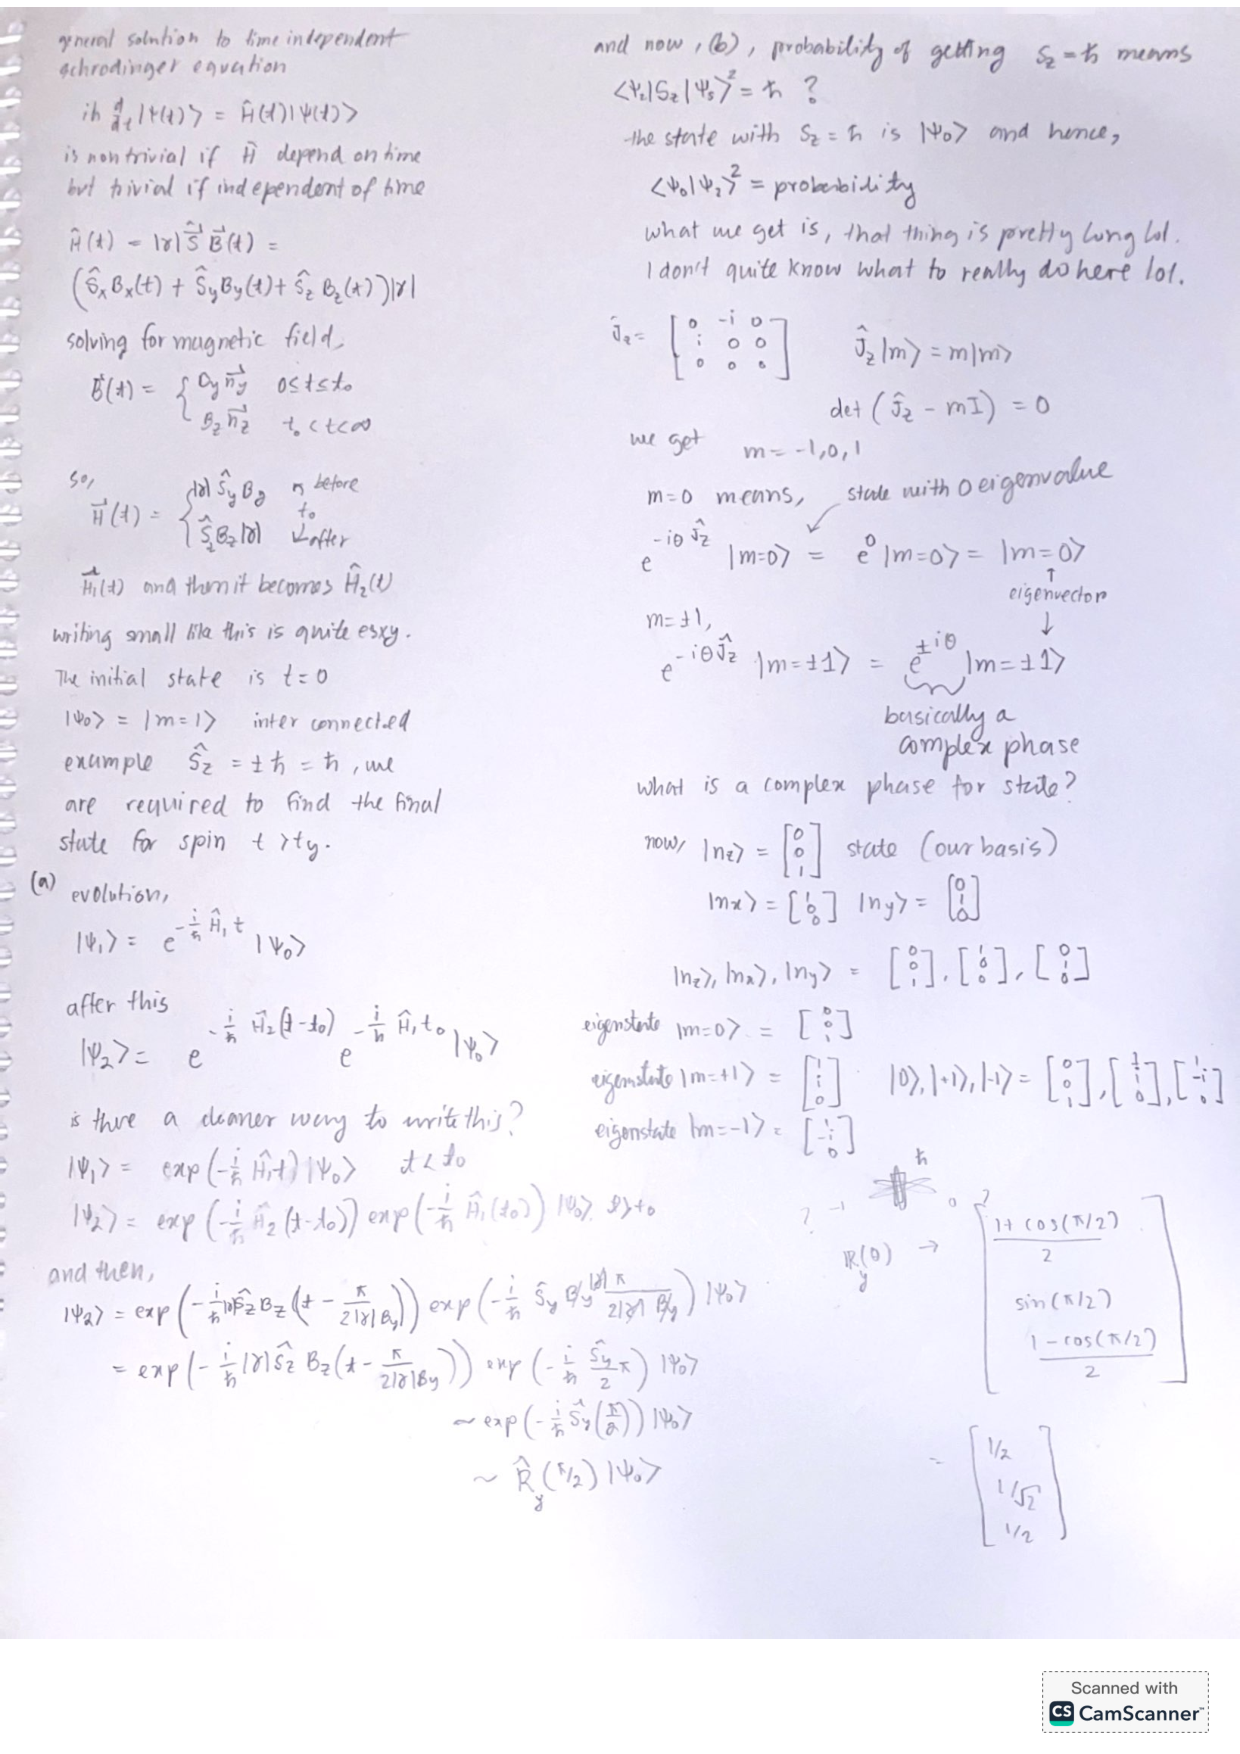
\includepdf[pages={1-}]{hw-7-hand.pdf}
\end{document}
